%!TEX root = ../../../main.tex

\subsection{MICAGes dataset}
    There does not exist a dataset publicly available in the literature which is dedicated to the evaluation of robustness of hand gesture recognition w.r.t. viewpoint changes.
    Therefore, thanks to the work of computer vision department at MICA Institute, a dataset was carefully designed and collected from multiple viewpoints in indoor environment with complex background.
    It consists of 9 dynamic hand gestures which correspond to control commands of electronic home appliances.
    Each gesture is a combination of hand movement following a pre-defined direction and changing of hand shape in a natural manner.

    Five Kinect sensors {K1, K2, K3, K4, K5} are setup at five positions in a square simulation room of $16m^2$ (Fig.\ref{Fig:MICAGes1}).
    This work aims to capture hand gestures under multiple viewpoints synchronously. The subjects are invited to stand at a fixed position approximately 2 meters in front of the center view.
    The Kinect sensors provide both RGB and Depth data recorded at frame rate of 20 fps and resolution of 640 $\times$ 480, which legitimates the capture a multi-view and multi-modal dataset.

    \begin{figure}[h]
        \centering
        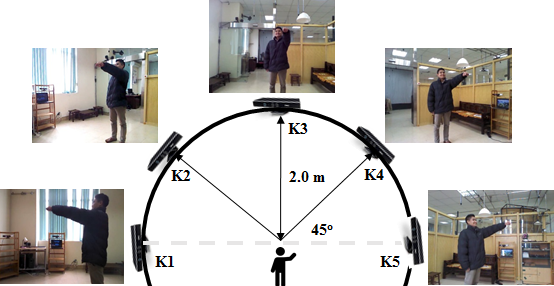
\includegraphics[width=0.8\linewidth]{figs/MICAGes1.png}
        \caption{Environment setup to capture MICAGes dataset.}
        %\vspace{-0.3cm}
        \label{Fig:MICAGes1}
    \end{figure}

    Twelve participants (08 males / 04 females) are voluntary to perform gestures one after another, each gesture three times.
    In the experiments of this thesis, only RGB information is concerned.
    Totally, the dataset contains 1620 (5 views $\times$ 9 gestures $\times$ 12 subjects $\times$ 3 times) dynamic hand gestures.
    Illustrations of segmented hand poses of a gesture are shown in Fig.\ref{Fig:MICAGes2}.

    \begin{figure}[htbp]
        \centering
        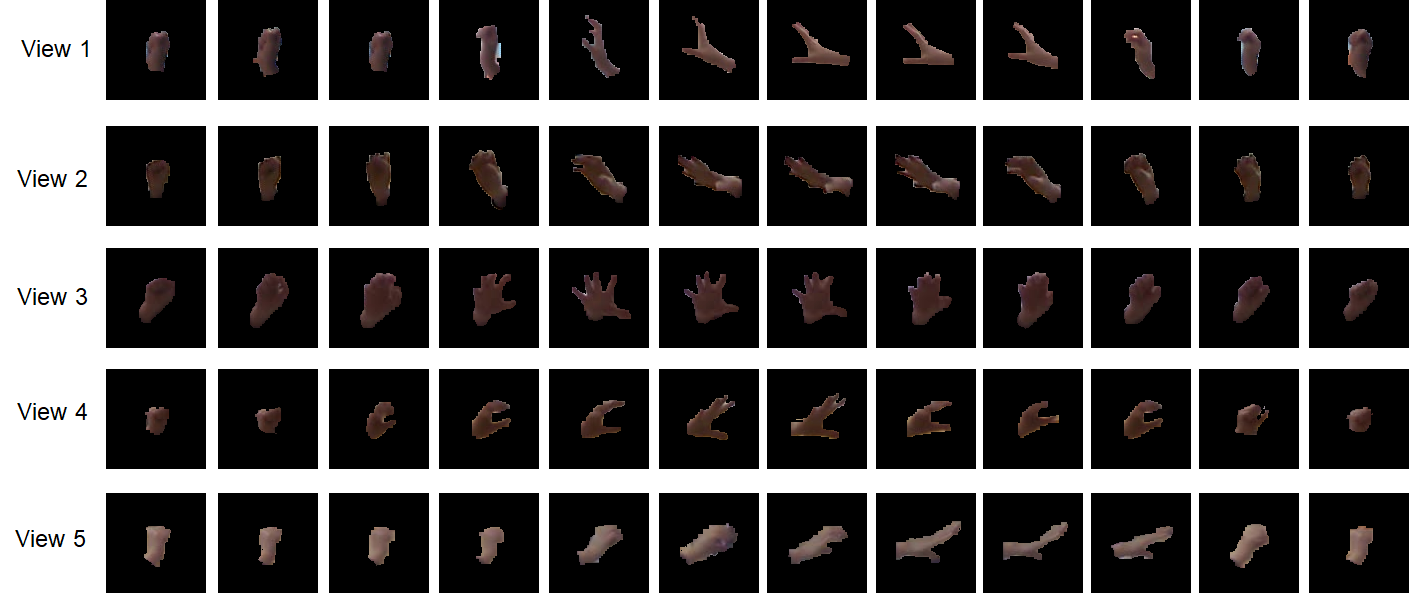
\includegraphics[width=0.9\linewidth]{figs/MICAGes2.png}
        \caption{Illustration of a gesture belonging to the $6^{th}$ class observed from 5 different views.}
        %\vspace{-0.3cm}
        \label{Fig:MICAGes2}
    \end{figure}
